\documentclass[30pt,twocolumn,letterpaper]{article}
\usepackage{cvpr}
\usepackage{times}
\usepackage{booktabs}
\usepackage{epsfig}
\usepackage{graphicx}
\usepackage{amsmath}
\usepackage{amssymb}
\cvprfinalcopy
\def\cvprPaperID{****}
\def\httilde{\mbox{\tt\raisebox{-.5ex}{\symbol{126}}}}
\usepackage{graphicx}
\usepackage{indentfirst}
\setlength{\parindent}{2em}
\usepackage{cite}
\usepackage[colorlinks,linkcolor=red,anchorcolor=blue,citecolor=green,backref=page]{hyperref}
\author{Qilei Zhang\\\\
Jun 6 2018}
\title{Stochastic Resonance Related Topics}
\begin{document}
\maketitle
\begin{abstract}
  In studying stochastic resonance, one looks at the periodic contribution of the output at the same frequency as the input. More recently, the general question of the generation of higher harmonics in the presence of noise has been addressed in a number of studies.
\end{abstract}
\section{Noise-induced Resonances}
Apart from numerical, adiabatic studies, an analytical theory allowing one to predict whether or not a particular system would exhibit noise-induced resonance has been put forward by Jung and Talkner. Their approach is sketched as follows: we consider here a general overdamped system subject to additive white noise and periodic forcing\cite{Barbay2000Experimental}.
\begin{figure}[htbp]
\small
\centering
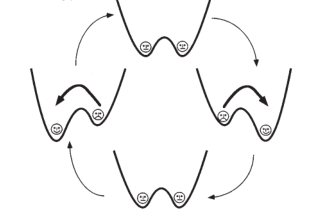
\includegraphics[width=20em]{000.png}
\caption{spatially extended systems}
\label{fig:lable}
\end{figure}
\section{Two coupled bistable systems}
The simplest way to study stochastic resonance in coupled systems is to consider two coupled overdamped bistable elements in the presence of noise and periodic forcing\cite{Adi1999Controlling}. \\
\begin{equation}
\quad x'=f(x)+A_0cos(wt+o)+u(t)
\end{equation}

\section{Periodically Rocked Molecular Motors}
It is generally appreciated that useful work cannot be extracted from thermal equilibrium fluctuations\cite{Wenning2003Activity}. Such a device would violate the second law of thermodynamics. Feynman et al. discussed this issue by means of a model of a mechanical ratchet��a scheme that was originally devised and elucidated during the heyday of early Brownian motion by M. V. Smoluchowski.
\section{Escape Rates In Periodically Driven Systems}
The problem of activated rates in threshold systems that are exposed to noise and periodic perturbations is nontrivial\cite{Lan2007Stochastic}.
{\small
\bibliographystyle{ieee}
\bibliography{1}
}
\end{document}
